% Sandia National Laboratories is a multimission laboratory managed and
% operated by National Technology & Engineering Solutions of Sandia, LLC, a
% wholly owned subsidiary of Honeywell International Inc., for the U.S.
% Department of Energy’s National Nuclear Security Administration under
% contract DE-NA0003525.

% Copyright 2002-2022 National Technology & Engineering Solutions of Sandia,
% LLC (NTESS).


\begin{Device}\label{V_DEVICE}

\symbol
{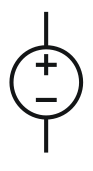
\includegraphics{ivsSymbol}}

\device
\begin{alltt}
V<name> <(+) node> <(-) node> [ [DC] <value> ]
+ [AC [magnitude value [phase value] ] ] [transient specification]
\end{alltt}

\examples
\begin{alltt}
VSLOW 1 22 SIN(0.5 1.0mV 1KHz 1ms)
VPULSE 1 3 PULSE(-1 1 2ns 2ns 2ns 50ns 100ns)
VPAT 2 4 PAT(5 0 0 1n 2n 5n b0101)
\end{alltt}


\parameters

\begin{Parameters}

\param{transient specification}

There are five predefined time-varying functions for sources:

\begin{description}
\item[\tt PULSE <parameters>] Pulse waveform
\item[\tt SIN <parameters>] Sinusoidal waveform
\item[\tt EXP <parameters>] Exponential waveform
\item[\tt PAT <parameters>] Pattern waveform
\item[\tt PWL <parameters>] Piecewise linear waveform
\item[\tt SFFM <parameters>] Frequency-modulated waveform
\end{description}

\end{Parameters}

\comments

Positive current flows from the positive node
through the source to the negative node. 

The power supplied or dissipated by the voltage source is calculated 
with $I \cdot \Delta V$ where the voltage drop is calculated as $(V_+ - V_-)$ 
and positive current flows from $V_+$ to $V_-$.  Dissipated power has a
positive sign, while supplied power has a negative sign.

None, any, or all of the DC, AC, and transient values
can be specified. The AC phase value is in degrees. 

\end{Device}

\paragraph{Transient Specifications}
This section outlines the available transient specifications. $\Delta t$ and
$T_{F}$ are the time step size and simulation end-time, respectively.
Parameters marked as -- must have a value specified for them;
otherwise a netlist parsing error will occur.

\subparagraph{Pulse}
\begin{alltt}
PULSE(V1 V2 TD TR TF PW PER)
\end{alltt}

\begin{DeviceParamTable}{Pulse Parameters}
V1 & Initial Value & Volt & -- \\ \hline
V2 & Pulse Value & Volt & 0.0 \\ \hline
TD & Delay Time & s & 0.0 \\ \hline
TR & Rise Time & s & $\Delta t$ \\ \hline
TF & Fall Time & s & $\Delta t$ \\ \hline
PW & Pulse Width & s & $T_F$ \\ \hline
PER & Period & s & $T_F$ \\ \hline
\end{DeviceParamTable}

\subparagraph{Sine}
\begin{alltt}
SIN(V0 VA FREQ TD THETA PHASE)
\end{alltt}

\begin{DeviceParamTable}{Sine Parameters}
V0 & Offset                & Volt & --   \\ \hline
VA & Amplitude             & Volt & --   \\ \hline
FREQ & Frequency           & s$^{-1}$  & --   \\ \hline
TD & Delay                 & s    & $\Delta t$ \\ \hline
THETA & Attenuation Factor & s    & $\Delta t$ \\ \hline
PHASE & Phase              & degrees & 0.0 \\ \hline 
\end{DeviceParamTable}

The waveform is shaped according to the following equations, where $\phi=\pi*\mathbf{PHASE}/180$ :
\[
V = \left\{ \begin{array}{ll}
V_0, & 0 < t < T_D \\
V_0 + V_A \sin[2\pi\cdot\mathbf{FREQ}\cdot(t - T_D)+\phi]
\exp[-(t - T_D) \cdot \mathbf{THETA}], & T_D < t < T_F
\end{array}
\right.
\]

\subparagraph{Exponent}
\begin{alltt}
EXP(V1 V2 TD1 TAU1 TD2 TAU2)
\end{alltt}

\begin{DeviceParamTable}{Exponent Parameters}
V1 & Initial Amplitude & Volt & -- \\ \hline
V2 & Amplitude & Volt & -- \\ \hline
TD1 & Rise Delay Time & s & 0.0 \\ \hline
TAU1 & Rise Time Constant & s & $\Delta t$ \\ \hline
TD2 & Delay Fall Time & s & TD1 $+ \Delta t$ \\ \hline
TAU2 & Fall Time Constant & s & $\Delta t$ \\ \hline
\end{DeviceParamTable}

The waveform is shaped according to the following equations:
\[
V = \left\{ \begin{array}{ll}
V_1, & 0 < t < \mathrm{TD1} \\
V_1 + (V_2 - V_1) \{1 - \exp[-(t-\mathrm{TD1}) / \mathrm{TAU1}] \} ,
& \mathrm{TD1} < t < \mathrm{TD2} \\
V_1 + (V_2 - V_1) \{1 - \exp[-(t- \mathrm{TD1}) / \mathrm{TAU1}] \} \\
\;\;\;\;\, + (V_1 - V_2) \{1 - \exp[-(t - \mathrm{TD2}) / \mathrm{TAU2}] \} ,
& \mathrm{TD2} < t < T_2
\end{array}
\right. \]

\subparagraph{Pattern}
\begin{alltt}
PAT(VHI VLO TD TR TF TSAMPLE DATA R)
\end{alltt}

\begin{DeviceParamTable}{Pattern Parameters}
VHI & High Value & Volt & -- \\ \hline
VLO & Low Value & Volt & -- \\ \hline
TD & Delay Time & s & -- \\ \hline
TR & Rise Time & s & -- \\ \hline
TF & Fall Time & s & -- \\ \hline
TSAMPLE & Bit period & s & -- \\ \hline
DATA & Bit pattern & -- & -- \\ \hline
R & Repeat & --  & 0 \\ \hline
\end{DeviceParamTable}

The \texttt{VHI}, \texttt{VLO}, \texttt{TD}, \texttt{TF}, \texttt{TF}
\texttt{TSAMPLE} and \texttt{DATA} parameters are all required, and
hence have no default values.  Negative values for \texttt{TD} are
supported.  The \texttt{R} parameter is optional.  For its default
value of 0, the requested bit pattern will occur once.

The \texttt{DATA} parameter is the requested bit-pattern.  Only the
0' and `1' states are supported.  The `M' and `Z' states are not
supported.  The \texttt{DATA} field should have a leading `b' (or `B')
character (e.g., be specified as `b0101' ).

For times earlier than \texttt{TD}, the waveform value is set by the
first bit in \texttt{DATA}.  For times after the end of the (possibly
repeated) pattern, the waveform value is set by the last bit in
\texttt{DATA}.  Piecewise linear interpolation is used to generate
the output value when transitioning between states.

The relationship between the various source parameters can be
illustrated with the following example:

V1 1 0 PAT(5 0 0 1n 1n 5n b010)

That V1 source definition would produce time-voltages pairs at
(0 0) (4.5ns 0) (5ns 2.5) (5.5ns 5.0) (9.5ns 5.0)
(10ns 2.5) (10.5ns 0).  So, the bit period is 5ns and the
voltage value at the start/end of each ``sample'' is equal to
0.5*(\texttt{VHI} + \texttt{VLO}).  The first rise is centered
around t=5ns, and hence starts at t=4.5ns and ends at t=5.5 ns.

The \texttt{VHI}, \texttt{VLO}, \texttt{TD}, \texttt{TF}, \texttt{TF}
and \texttt{TSAMPLE} parameters are compatible with \texttt{.STEP}.
The \texttt{DATA} and \texttt{R} parameters are not.

The HSPICE parameters \texttt{RB}, \texttt{ENCODE} and \texttt{RD\_INIT},
for the pattern source, are not supported.

\subparagraph{Piecewise Linear}
\begin{alltt}
PWL  T0 V0 [Tn Vn]*
PWL  FILE "<name>" [TD=<timeDelay>] [R=<repeatTime>]
\end{alltt}

\begin{DeviceParamTable}{Piecewise Linear Parameters}
T$_n$ & Time at Corner & s & none \\ \hline
V$_n$ & Voltage at Corner & Volt & none \\ \hline
TD & Time Delay & s & 0 \\ \hline
R & Repeat Time & s & none \\ \hline 
\end{DeviceParamTable}

When the FILE option is given, \Xyce{} will read the corner points
from the file specified in the \texttt{<name>} field.  This file
should be a plain ASCII text file (or a .CSV file) with time/voltage pairs.  
There should be one pair per line, and the time and voltage values should be
separated by whitespace or commas. As an example, the file 
specified (e.g., \texttt{vpwl.csv}) could have these five lines:
\begin{alltt}
0.00, 0.00
2.00, 3.00
3.00, 2.00
4.00, 2.00
4.01, 5.00
\end{alltt}
The corresponding example instance lines would be:
\begin{alltt}
VPWL1 1 0 PWL 0S 0V  2S 3V  3S 2V  4S 2V  4.01S 5V
VPWL2 2 0 PWL FILE "vpwl.txt"
VPWL3 3 0 PWL file "vpwl.csv"
VPWL4 4 0 PWL FILE vpwl.csv
\end{alltt}

The double quotes around the file name are optional, as shown above.

It is a best practice to specify all of the time-voltage pairs in the PWL specification.
However, for compatibility with HSPICE and PSpice, if the user-specified list of 
time/voltage pairs omits the pair at time=0 as the first pair in the list then \Xyce{} 
will insert a pair at time=0 with the voltage value at the first user-specified time value.  
As an example, this user-specified list:
\begin{alltt}
2S 3V  3S 2V  4S 2V  4.01S 5V
\end{alltt}
would be implemented in \Xyce{} as follows:  
\begin{alltt} 
0S 3V  2S 3V  3S 2V  4S 2V  4.01S 5V
\end{alltt}

TD has units of seconds, and specifies the length of time to delay
the start of PWL waveform.  The default is to have no delay, and TD is 
an optional parameter.

The Repeat Time (R) is an optional parameter.  If R is omitted then the waveform
will not repeat.  If R is included then the waveform will repeat until the end
of the simulation.  As examples, R=0 means repeat the PWL waveform from time=0
to the last time (T$_N$) specified in the waveform specification. (This would use the
time points 0s, 2s, 3s, 4s and 4.01s for the example waveform given above.)
In general, R=\texttt{<repeatTime>} means repeat the waveform from time equal to
\texttt{<repeatTime>} seconds in the waveform specification to the last time (T$_N$)
specified in the waveform specification.  So, the \texttt{<repeatTime>} must be 
greater than or equal to 0 and less than the last time point (T$_N$).
If the R parameter is used then it must have a value.  

The specification \texttt {PWL  FILE "<name>"  R}  \texttt is illegal in \Xyce{} as
a shorthand for R=0.  Also, the \Xyce{} syntax for PWL sources is not compatible
with the PSpice \texttt{REPEAT} syntax for PWL sources. See section 
\ref{PWL_SOURCE_SYNTAX_DIFF} for more details.

The repeat time (R) does enable the specification of discontinuous piecewise linear
waveforms.  For example, this waveform is a legal \Xyce{} syntax.  
\begin{alltt}
VPWL1 1 0 PWL 0S 0V  2S 3V  3S 2V  4S 2V  4.01V 5V  R=2
\end{alltt}
However, in general, discontinuous source waveforms may cause convergence problems.

\subparagraph{Frequency Modulated}
\begin{alltt}
SFFM (V0 VA FC MDI FS)
\end{alltt}

\begin{DeviceParamTable}{Frequency Modulated Parameters}
V0 & Offset & Volt & -- \\ \hline
VA & Amplitude & Volt & -- \\ \hline
FC & Carrier Frequency & hertz & 1/\textrmb{TSTOP} \\ \hline
MDI & Modulation Index & - & 0 \\ \hline
FS & Signal Frequency & hertz & 1/\textrmb{TSTOP} \\ \hline
\end{DeviceParamTable}

\textrmb{TSTOP} is the final time, as entered into the transient
(\texttt{.TRANS}) command. The waveform is shaped according to the following
equation:
\[
V = {V_0 + V_A} \cdot \sin(2\pi \cdot \mathrm{FC} \cdot \mathbf{TIME} +
\mathrm{MDI} \cdot \sin(2\pi \cdot \mathrm{FS} \cdot \mathbf{TIME}))
\]
where \textrmb{TIME} is the current simulation time.
